\documentclass{beamer}
\beamertemplatenavigationsymbolsempty
\usecolortheme{beaver}
\setbeamertemplate{blocks}[rounded=true, shadow=true]
\setbeamertemplate{footline}[page number]
%
\usepackage[utf8]{inputenc}
\usepackage[english]{babel}
\usepackage{amssymb,amsfonts,amsmath,mathtext}
\usepackage{subfig}
\usepackage[all]{xy} % xy package for diagrams
\usepackage{array}
\usepackage{multicol}% many columns in slide
\usepackage{hyperref}% urls
\usepackage{hhline}%tables
% Your figures are here:
\graphicspath{ {fig/} {../fig/} }

%----------------------------------------------------------------------------------------------------------
\title[\hbox to 56mm{Feature generation}]{Winterstorm prediction}
\author[N.\,M.~Kornilov]{Nikita Kornilov}
\institute{Moscow Institute of Physics and Technology}
\date{\footnotesize
\par\smallskip\emph{Course:} My first scientific paper\par (Strijov's practice)/Group 904 %821, 813
\par\smallskip\emph{Expert:} Y.~Maximov
\par\bigskip\small 2022}

%----------------------------------------------------------------------------------------------------------
\begin{document}
%----------------------------------------------------------------------------------------------------------
\begin{frame}
\thispagestyle{empty}
\maketitle
\end{frame}
%-----------------------------------------------------------------------------------------------------
%\begin{frame}{Goal of research}
%..
%\end{frame}
%-----------------------------------------------------------------------------------------------------
\begin{frame}{One-slide talk}
\begin{columns}
\column{0.4\textwidth}
\qquad $(24, 64)$ class and feature maps example
\column{0.8\textwidth}
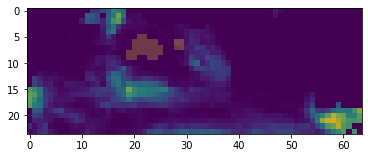
\includegraphics[width=0.5\textwidth]{fig/image sample.png}
\end{columns}

\textbf{Goal: predict both maps in time t} 

Model structure 
\begin{columns}[c]
\column{0.5\textwidth}
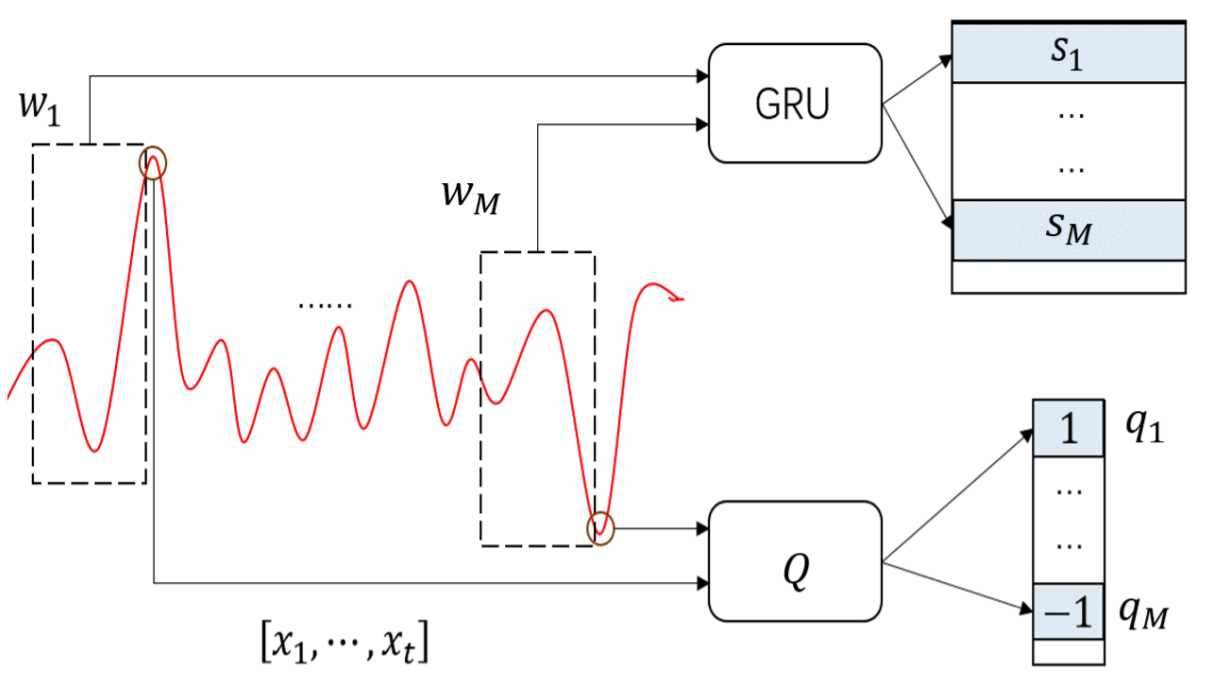
\includegraphics[width=0.7\textwidth]{fig/memory module.png}
    
\column{0.6\textwidth}
    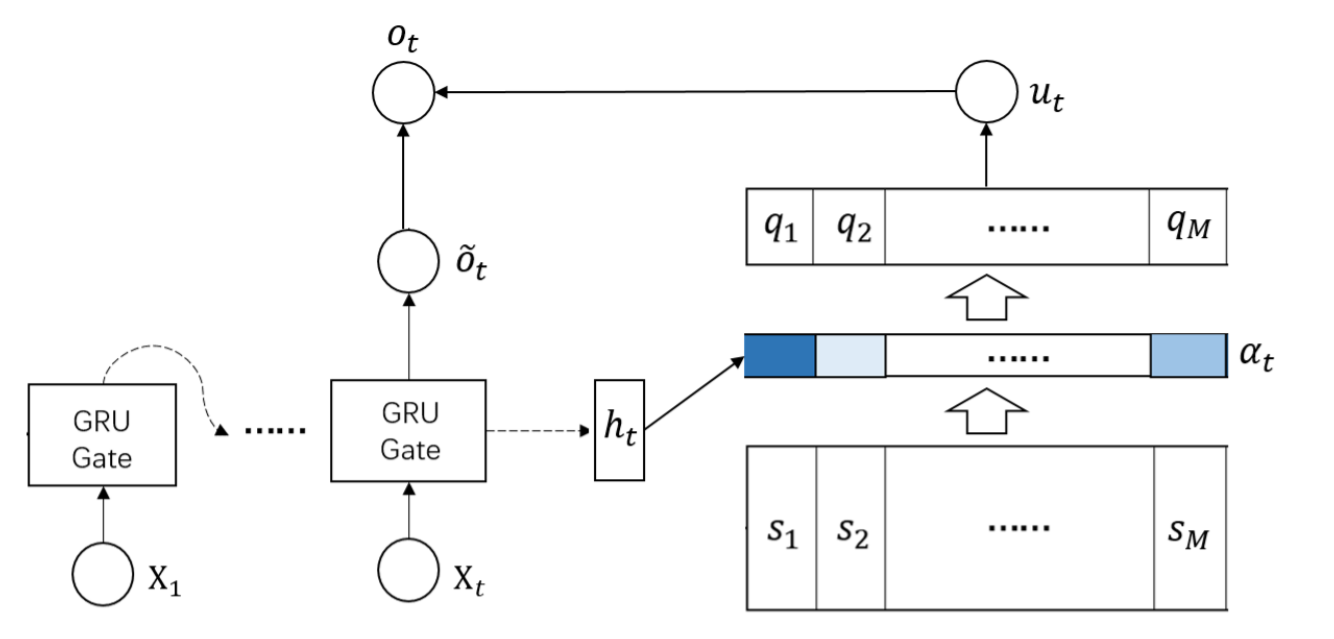
\includegraphics[width=0.7\textwidth]{fig/attention.png}

\end{columns}
\bigskip
\begin{columns}[c]
\column{0.7\textwidth}
\qquad Extreme Value Loss or EVL with $\gamma$
\bigskip


 $\textit{EVL}(u_t,v_t) = -\beta_0 \left( 1 - \frac{u_t}{\gamma}\right)^\gamma v_t\log(u_t) $  
 $ -\beta_1 \left( 1 - \frac{1 - u_t}{\gamma}\right)^\gamma (1-v_t)\log(1 - u_t) $ 


\bigskip
\qquad $\beta_i = Pr(v_t = i ),  i \in \{0,1\}$
\column{0.4\textwidth} 
Total loss

$  ||o_t - y_t||^2_F +  \lambda \textit{EVL}(u_t, v_t)$

\bigskip
$o_t$ - predicted feature map $u_t$ - predicted class map 
\qquad $\lambda$ - hyperparameter

\end{columns}
\end{frame}


%----------------------------------------------------------------------------------------------------------
%\begin{frame}{Problem statement}
%..
%\end{frame}
%----------------------------------------------------------------------------------------------------------
%\begin{frame}{Solution}
%\begin{columns}[c]
%\column{0.6\textwidth}
%    Column 1
%\column{0.4\textwidth}
%    Column 2
%\end{columns}
%\end{frame}
%----------------------------------------------------------------------------------------------------------
%\begin{frame}{Computational experiment}
%..
%\end{frame}
%----------------------------------------------------------------------------------------------------------
%\begin{frame}{Conclusion}
 %   \begin{block}{Forecast with hierarchical aggregation of}
 %   \begin{itemize}
 %       \item types of freight in
 %       \item stations, regions, and roads,
 %       \item for a day, week, month, and quarter.
 %  \end{block}
%\end{frame}
%----------------------------------------------------------------------------------------------------------

\end{document} 